% --------------------------------------------------
% Post-CFET Device Architecture Paper (English Version)
% --------------------------------------------------
\documentclass[conference]{IEEEtran}
\IEEEoverridecommandlockouts

% Packages
\usepackage{graphicx}
\usepackage{amsmath,amssymb}
\usepackage{hyperref}
\usepackage{booktabs}
\usepackage{multirow}
\usepackage{url}
\usepackage{standalone}   % for \includestandalone
% --- TikZ 共通設定(追加) ---
\usepackage{tikz}
\usetikzlibrary{shapes,arrows.meta,positioning,fit,mindmap,calc}
% 図で使う共通スタイル
\tikzset{
  blk/.style={rectangle,rounded corners,draw=black,fill=blue!10,
              minimum width=2.8cm,minimum height=0.8cm,align=center},
  flowarrow/.style={-{Latex[length=3mm,width=2mm]},thick},
  mod/.style={rectangle,draw=black,fill=white,
              minimum width=2.4cm,minimum height=0.8cm,align=center},
  title/.style={font=\bfseries},
  bubble/.style={draw, rounded corners, fill=blue!7, align=left,
                 inner sep=2.5pt, font=\scriptsize},
  milestone/.style={circle, draw, fill=black, minimum size=2pt, inner sep=0pt},
  arrow/.style={-{Latex[length=3mm,width=2mm]}, thick}
}

% --------------------------------------------------
% Title & Author
% --------------------------------------------------
\title{Post-CFET Device Architectures: Materials, Integration, and Design Perspectives}

\author{
\IEEEauthorblockN{Shinichi Samizo}
\IEEEauthorblockA{Independent Semiconductor Researcher\\
Project Design Hub, Samizo-AITL\\
\textit{Email:} \href{mailto:shin3t72@gmail.com}{shin3t72@gmail.com}\\
\textit{GitHub:} \href{https://github.com/Samizo-AITL}{Samizo-AITL}}
}

\begin{document}
\maketitle

% --------------------------------------------------
% Abstract
% --------------------------------------------------
\begin{abstract}
CMOS scaling has evolved from Planar MOSFETs to FinFETs, Gate-All-Around (GAA) nanosheets, and Complementary FETs (CFETs). CFET improves electrostatic control and mitigates wiring bottlenecks, but silicon is approaching its material and thermal limits. This paper reviews \textbf{post-CFET device candidates} including \textit{two-dimensional (2D) material FETs, monolithic 3D integration, spintronics/quantum devices, and heterogeneous atomic-scale integration}. Their physical principles, fabrication challenges, experimental demonstrations, reliability concerns, application domains, and implications for design and education are compared.
\end{abstract}

% --------------------------------------------------
% Introduction
% --------------------------------------------------
\section{Introduction}
The semiconductor industry has advanced for more than five decades through device scaling and structural innovation. 
The trajectory from Planar MOSFET $\to$ FinFET $\to$ GAA $\to$ CFET represents the pursuit of enhanced electrostatic control and integration efficiency.  
However, mobility degradation, leakage, wiring delay, and thermal density have become limiting factors, demanding exploration of \textbf{post-CFET technologies}.

% --------------------------------------------------
% Evolution Path
% --------------------------------------------------
\section{Evolution from CMOS to Post-CFET}
Fig.~\ref{fig:evolution} shows the historical pathway of CMOS device evolution.

\begin{figure}[t]
  \centering
  \documentclass[tikz,border=5pt]{standalone}
\usetikzlibrary{shapes,arrows.meta,positioning}

% NOTE: don't use style name 'node' (reserved). Use 'blk'.
\tikzset{
  blk/.style={rectangle,rounded corners,draw=black,fill=blue!10,
              minimum width=2.8cm,minimum height=0.8cm,align=center},
  flowarrow/.style={-{Latex[length=3mm,width=2mm]},thick}
}

\begin{document}
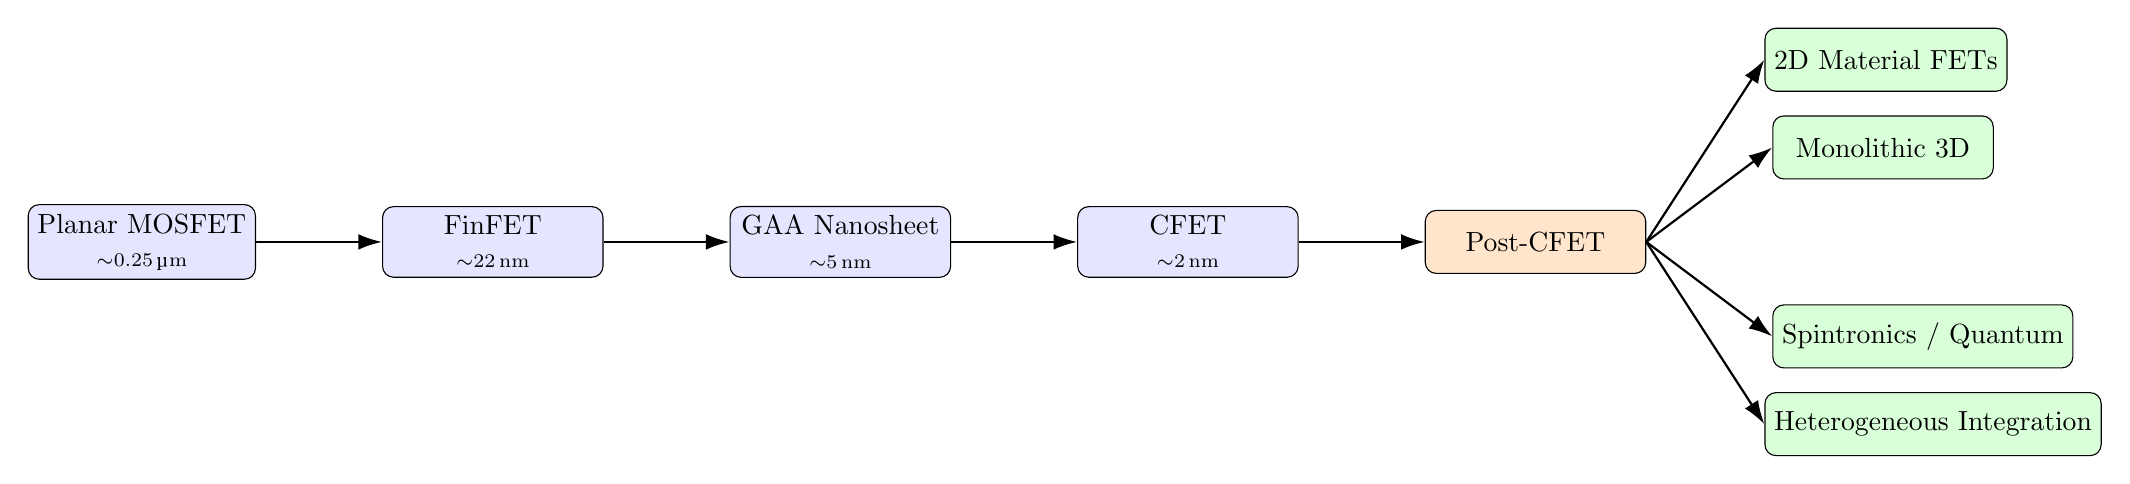
\begin{tikzpicture}[node distance=1.6cm]
  \node[blk] (planar) {Planar MOSFET \\ \scriptsize $\sim$0.25\,\textmu m};
  \node[blk, right=of planar] (finfet) {FinFET \\ \scriptsize $\sim$22\,nm};
  \node[blk, right=of finfet] (gaa) {GAA Nanosheet \\ \scriptsize $\sim$5\,nm};
  \node[blk, right=of gaa] (cfet) {CFET \\ \scriptsize $\sim$2\,nm};
  \node[blk, right=of cfet, fill=orange!20] (post) {Post-CFET};

  \draw[flowarrow] (planar) -- (finfet);
  \draw[flowarrow] (finfet) -- (gaa);
  \draw[flowarrow] (gaa) -- (cfet);
  \draw[flowarrow] (cfet) -- (post);

  % Branches
  \node[blk, above right=1.5cm and 1.5cm of post, fill=green!15] (f2d) {2D Material FETs};
  \node[blk, right=of post, yshift=1.2cm, fill=green!15] (m3d) {Monolithic 3D};
  \node[blk, right=of post, yshift=-1.2cm, fill=green!15] (spin) {Spintronics / Quantum};
  \node[blk, below right=1.5cm and 1.5cm of post, fill=green!15] (hetero) {Heterogeneous Integration};

  \draw[flowarrow] (post.east) -- (f2d.west);
  \draw[flowarrow] (post.east) -- (m3d.west);
  \draw[flowarrow] (post.east) -- (spin.west);
  \draw[flowarrow] (post.east) -- (hetero.west);
\end{tikzpicture}
\end{document}

  \caption{Evolution tree: CMOS $\to$ CFET $\to$ Post-CFET candidates.}
  \label{fig:evolution}
\end{figure}

\subsection{Planar MOSFET to FinFET}
Short-channel effects and leakage became critical below 45 nm. Tri-gate FinFETs improved gate control and became the industry standard.

\subsection{FinFET to GAA}
Cell height constraints required nanosheets fully surrounded by gates. GAA provides stronger electrostatics but increases process variability.

\subsection{GAA to CFET}
CFET vertically stacks nFET and pFET, improving cell density and reducing interconnect delay. Challenges include heat removal and process complexity.

\subsection{Beyond CFET}
Silicon material limits and wiring dominance demand novel materials, new integration schemes, and alternative state variables (spin, photon, bio).

% --------------------------------------------------
% Candidate Technologies
% --------------------------------------------------
\section{Post-CFET Candidate Technologies}

\subsection{2D Material FETs}
\begin{itemize}
  \item \textbf{Demonstrations:} MoS$_2$ FET ($L_g$=12 nm, IEDM 2023) with Ion/Ioff=$10^7$, SS=65 mV/dec. 
  \item \textbf{Challenges:} High contact resistance ($R_c \approx 1$ k$\Omega\cdot\mu$m), film non-uniformity (5--10\%), interface traps.  
  \item \textbf{Applications:} Ultra-low power IoT, flexible electronics, bio-sensing.  
  \item \textbf{Design impact:} Immature SPICE models, poor statistical variability data.  
\end{itemize}

\subsection{Monolithic 3D Integration (M3D)}
\begin{itemize}
  \item \textbf{Demonstrations:} SRAM stacking (IEDM 2019): delay -30\%, area -40\%. AI SoC (Nat. Electronics 2022): energy efficiency +1.7$\times$.  
  \item \textbf{Challenges:} Low-temperature processing ($<450^\circ$C), inter-layer $V_{th}$ variation, thermal hotspots $>1$ W/mm$^2$.  
  \item \textbf{Applications:} AI accelerators, memory-centric computing.  
  \item \textbf{Design impact:} Requires 3D P\&R EDA, thermal/mechanical co-simulation.  
\end{itemize}

\subsection{Spintronics / Quantum Devices}
\begin{itemize}
  \item \textbf{Demonstrations:} STT-MRAM endurance $10^{12}$ cycles (IBM), SOT-MRAM write current -40\%, Topological FET on/off=$10^3$ at RT.  
  \item \textbf{Challenges:} CMOS compatibility, reducing write current from mA to $\mu$A.  
  \item \textbf{Applications:} Neuromorphic computing, radiation-hardened space systems, in-memory logic.  
  \item \textbf{Design impact:} Logic-memory fusion beyond von Neumann architecture.  
\end{itemize}

\subsection{Heterogeneous Atomic-Scale Integration}
\begin{itemize}
  \item \textbf{Demonstrations:} Si + MoS$_2$ photodetector, responsivity 200 mA/W @ 1.55 $\mu$m (Nat. Photonics 2020). CMOS+MEMS sensor chips.  
  \item \textbf{Challenges:} Interface stability, lattice/thermal mismatch, yield.  
  \item \textbf{Applications:} Optical interconnect, medical sensing, aerospace.  
  \item \textbf{Design impact:} Cross-domain EDA required (electrical + optical + mechanical).  
\end{itemize}

% --------------------------------------------------
% Block diagram
% --------------------------------------------------
\begin{figure}[t]
  \centering
  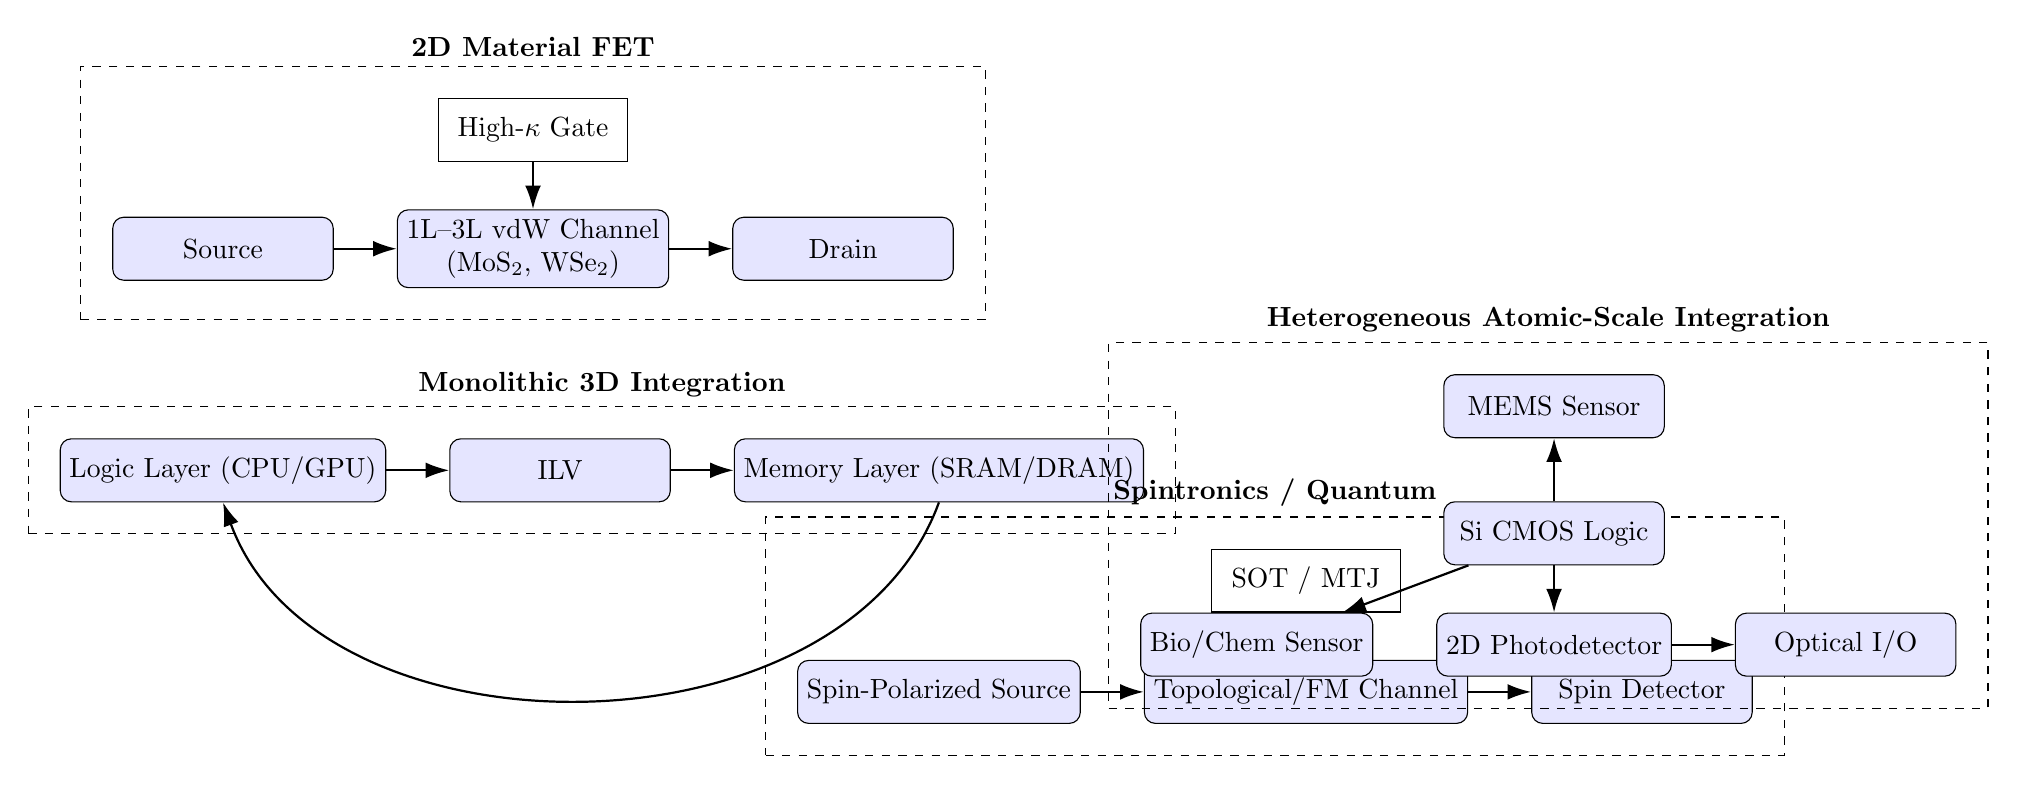
\begin{tikzpicture}[node distance=6mm and 8mm]
% --- 2D FET ---
\node[blk] (src) {Source};
\node[blk, right=of src] (chan) {1L--3L vdW Channel\\ (MoS$_2$, WSe$_2$)};
\node[blk, right=of chan] (drn) {Drain};
\node[mod, above=6mm of chan] (gate) {High-$\kappa$ Gate};
\draw[arrow] (src) -- (chan);
\draw[arrow] (chan) -- (drn);
\draw[arrow] (gate) -- (chan);
\node[draw=black, dashed, inner sep=4mm, fit=(src)(chan)(drn)(gate),
      label={[title]above:2D Material FET}] {};

% --- M3D ---
\node[blk, below=20mm of src] (logic) {Logic Layer (CPU/GPU)};
\node[blk, right=of logic] (ilv) {ILV};
\node[blk, right=of ilv] (mem) {Memory Layer (SRAM/DRAM)};
\draw[arrow] (logic) -- (ilv);
\draw[arrow] (ilv) -- (mem);
\draw[arrow] (mem.south) to[out=-110,in=-70] (logic.south);
\node[draw=black, dashed, inner sep=4mm, fit=(logic)(ilv)(mem),
      label={[title]above:Monolithic 3D Integration}] {};

% --- Spintronics / Quantum ---
\node[blk, below=20mm of mem] (spin_src) {Spin-Polarized Source};
\node[blk, right=of spin_src] (spin_ch) {Topological/FM Channel};
\node[blk, right=of spin_ch] (spin_det) {Spin Detector};
\node[mod, above=6mm of spin_ch] (sot) {SOT / MTJ};
\draw[arrow] (spin_src) -- (spin_ch);
\draw[arrow] (spin_ch) -- (spin_det);
\draw[arrow] (sot) -- (spin_ch);
\node[draw=black, dashed, inner sep=4mm, fit=(spin_src)(spin_ch)(spin_det)(sot),
      label={[title]above:Spintronics / Quantum}] {};

% --- Heterogeneous Integration ---
\node[blk, right=38mm of mem, yshift=-8mm] (cmos) {Si CMOS Logic};
\node[blk, below=of cmos] (pd) {2D Photodetector};
\node[blk, right=of pd] (optio) {Optical I/O};
\node[blk, above=of cmos, yshift=2mm] (mems) {MEMS Sensor};
\node[blk, left=of pd] (bio) {Bio/Chem Sensor};
\draw[arrow] (cmos) -- (pd);
\draw[arrow] (pd) -- (optio);
\draw[arrow] (cmos) -- (mems);
\draw[arrow] (cmos) -- (bio);
\node[draw=black, dashed, inner sep=4mm, fit=(cmos)(pd)(optio)(mems)(bio),
      label={[title]above:Heterogeneous Atomic-Scale Integration}] {};
\end{tikzpicture}

  \caption{Conceptual block diagrams of candidate device/integration options.}
\end{figure}

% --------------------------------------------------
% Mindmap
% --------------------------------------------------
\begin{figure}[t]
  \centering
  % figures/mindmap.tex — clean pro look (no mindmap lib)
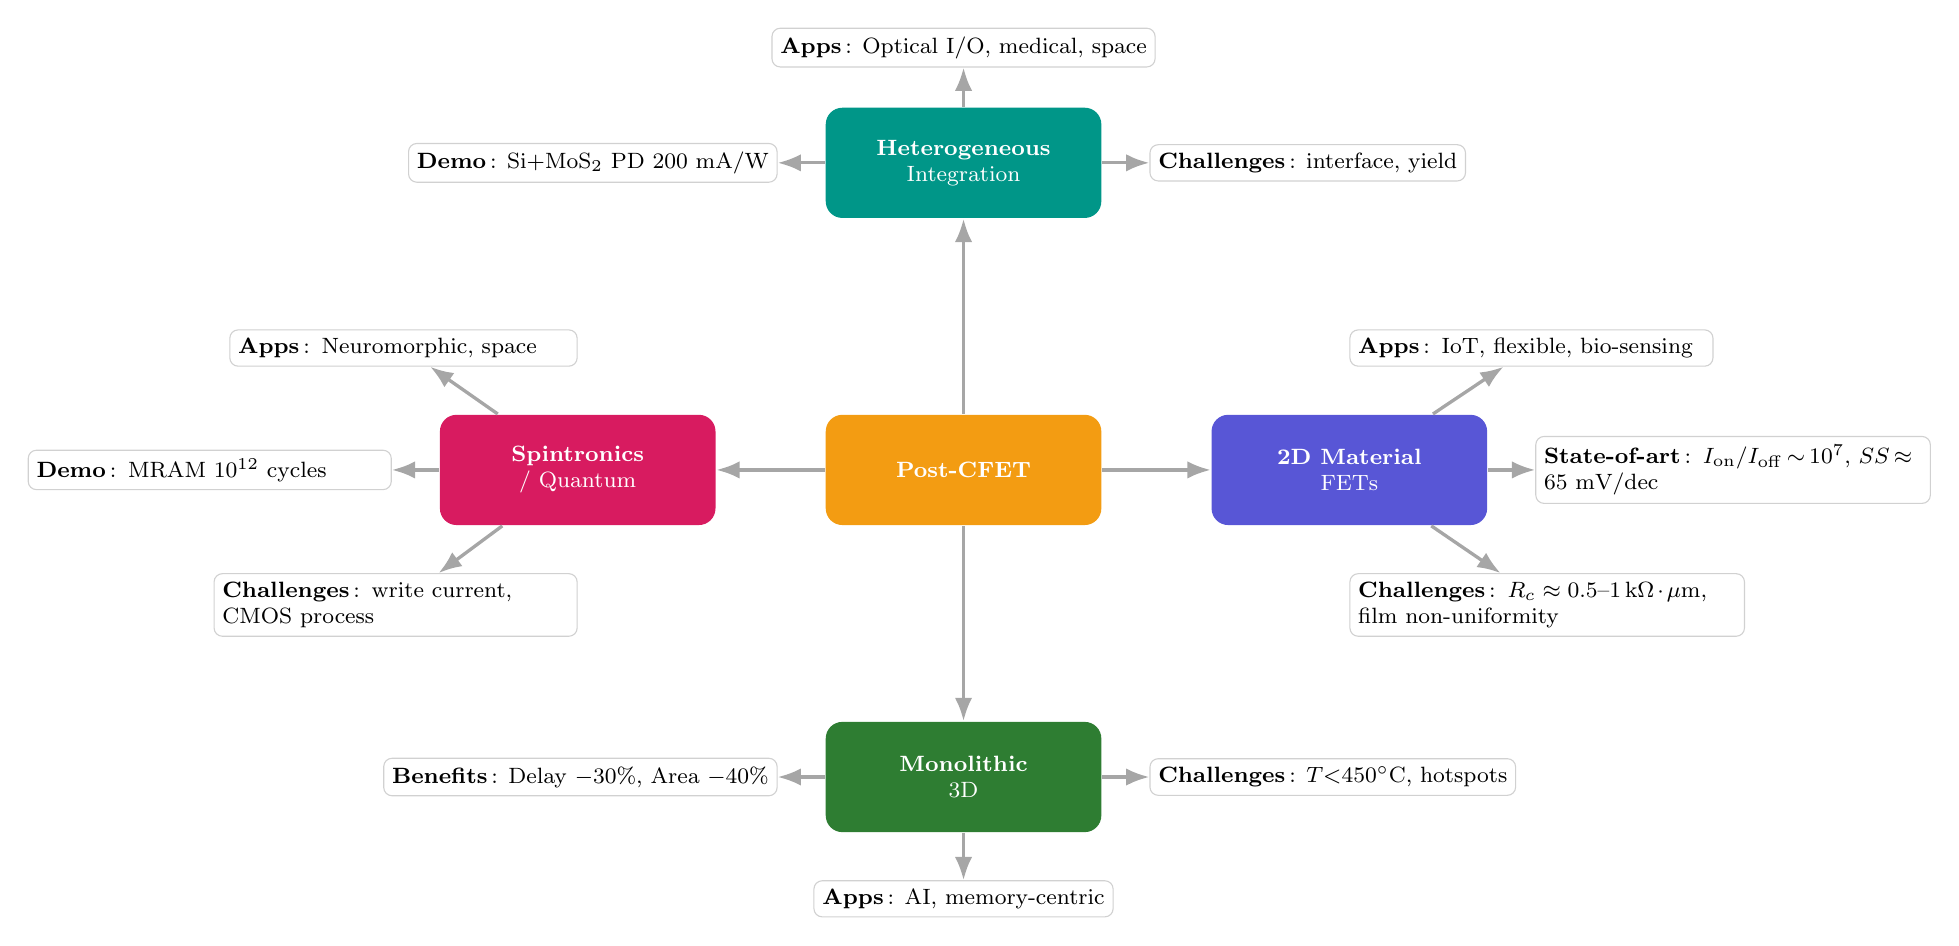
\begin{tikzpicture}[
  %----- styles -----
  font=\footnotesize,
  >=Latex,
  card/.style={
    draw=black!18, rounded corners=3pt, fill=white, align=left,
    inner sep=3pt, minimum width=38mm
  },
  topic/.style={
    rounded corners=6pt, align=center, text=white, semithick,
    minimum width=35mm, minimum height=14mm
  },
  link/.style={-Latex, very thick, draw=black!35},
  dot/.style={circle, fill=black!35, inner sep=1pt}
]
%----- palette (淡色で印刷も可) -----
\definecolor{cCore}{RGB}{243,156,18}   % orange
\definecolor{c2D}{RGB}{88, 86,214}     % blue-violet
\definecolor{cM3D}{RGB}{46,125,50}     % green
\definecolor{cSpin}{RGB}{216,27,96}    % magenta
\definecolor{cHet}{RGB}{0,150,136}     % teal

%----- layout points -----
\node[topic, fill=cCore] (core) at (0,0) {\bfseries Post-CFET};

\node[topic, fill=cHet]  (het)  at (0, 3.9) {\bfseries Heterogeneous\\ Integration};
\node[topic, fill=c2D]   (twod) at (4.9,0) {\bfseries 2D Material\\ FETs};
\node[topic, fill=cM3D]  (m3d)  at (0,-3.9) {\bfseries Monolithic\\ 3D};
\node[topic, fill=cSpin] (spin) at (-4.9,0) {\bfseries Spintronics\\ / Quantum};

% connectors from center
\draw[link] (core) -- (het);
\draw[link] (core) -- (twod);
\draw[link] (core) -- (m3d);
\draw[link] (core) -- (spin);

%----- Heterogeneous cards (top) -----
\node[card, above=5mm of het]   (h-app) {\textbf{Apps}\,: Optical I/O, medical, space};
\node[card, left=6mm  of het]   (h-demo){\textbf{Demo}\,: Si+MoS$_2$ PD 200 mA/W};
\node[card, right=6mm of het]   (h-ch)  {\textbf{Challenges}\,: interface, yield};
\foreach \x in {h-app,h-demo,h-ch} {\draw[link] (het) -- (\x);}

%----- 2D FETs cards (right) -----
\node[card, above=6mm of twod, anchor=south west, text width=44mm] (d-app)
  {\textbf{Apps}\,: IoT, flexible, bio-sensing};
\node[card, right=6mm of twod, anchor=west, text width=48mm] (d-ion)
  {\textbf{State-of-art}\,: $I_{\rm on}/I_{\rm off}\!\sim\!10^7$, $SS\!\approx\!65$ mV/dec};
\node[card, below=6mm of twod, anchor=north west, text width=48mm] (d-ch)
  {\textbf{Challenges}\,: $R_c\!\approx\!0.5$–$1\,\mathrm{k}\Omega\!\cdot\!\mu$m, film non-uniformity};
\foreach \x in {d-app,d-ion,d-ch} {\draw[link] (twod) -- (\x);}

%----- M3D cards (bottom) -----
\node[card, below=6mm of m3d] (m-app) {\textbf{Apps}\,: AI, memory-centric};
\node[card, left=6mm  of m3d] (m-perf){\textbf{Benefits}\,: Delay $-30\%$, Area $-40\%$};
\node[card, right=6mm of m3d] (m-ch)  {\textbf{Challenges}\,: $T{<}450^{\circ}$C, hotspots};
\foreach \x in {m-app,m-perf,m-ch} {\draw[link] (m3d) -- (\x);}

%----- Spin/Quantum cards (left) -----
\node[card, above=6mm of spin, anchor=south east, text width=42mm] (s-app)
  {\textbf{Apps}\,: Neuromorphic, space};
\node[card, left=6mm of spin, anchor=east, text width=44mm]   (s-mram)
  {\textbf{Demo}\,: MRAM $10^{12}$ cycles};
\node[card, below=6mm of spin, anchor=north east, text width=44mm] (s-ch)
  {\textbf{Challenges}\,: write current, CMOS process};
\foreach \x in {s-app,s-mram,s-ch} {\draw[link] (spin) -- (\x);}

% small dots at topic midpoints (飾り)
\foreach \n in {het,twod,m3d,spin} \fill[dot] (\n) circle (0pt);
\end{tikzpicture}

  \caption{Post-CFET technology mind map.}
\end{figure}

% --------------------------------------------------
% Comparison Table
% --------------------------------------------------
\section{Comparison Matrix}
Table~\ref{tab:matrix} compares the four candidate technologies.

\begin{table}[ht]
\centering
\caption{Comparison of Post-CFET candidate technologies}
\label{tab:matrix}
\begin{tabular}{lccccc}
\toprule
Tech. & Demonstrations & Rc/Thermal & Reliability & Applications & TRL \\
\midrule
2D-FET & Ion/Ioff=1e7 & 1k$\Omega\mu$m & Film variation & IoT/Flex & 3--5 \\
M3D & Delay-30\% & $<450^\circ$C & $V_{th}$ shift & AI/Memory & 4--6 \\
Spin & MRAM 1e12 cyc & RT stability & Write stress & Neuro/Space & 3--5 \\
Hetero & Si+MoS$_2$ PD & Interface limits & Yield & Optics/Med & 2--4 \\
\bottomrule
\end{tabular}
\end{table}

% --------------------------------------------------
% Roadmap
% --------------------------------------------------
\begin{figure}[t]
  \centering
  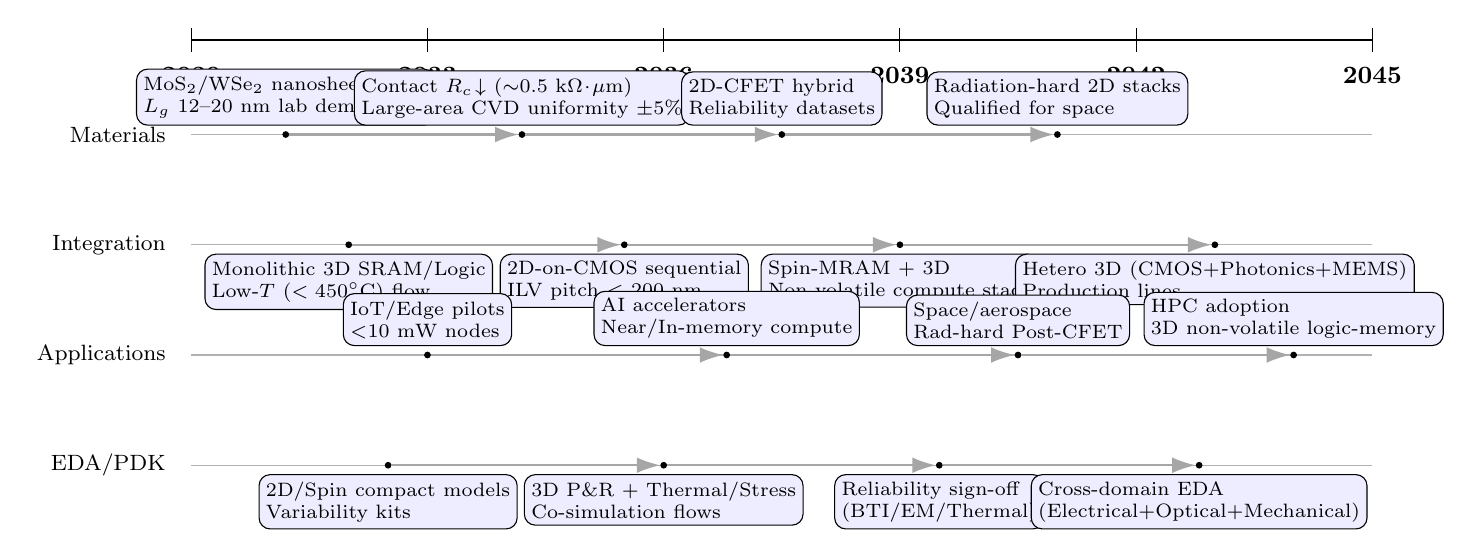
\begin{tikzpicture}[
  >=LaTeX,
  year/.style={font=\bfseries\small},
  lane/.style={font=\footnotesize,align=left}
]
% Axis
\draw[thick] (0,0) -- (15,0);
\foreach \x/\y in {0/2030,3/2033,6/2036,9/2039,12/2042,15/2045} {
  \draw (\x,0.15) -- (\x,-0.15) node[below=2pt,year] {\y};
}

% Lanes
\node[lane, anchor=east] at (-0.2, -1.2) {Materials};
\node[lane, anchor=east] at (-0.2, -2.6) {Integration};
\node[lane, anchor=east] at (-0.2, -4.0) {Applications};
\node[lane, anchor=east] at (-0.2, -5.4) {EDA/PDK};
\draw[gray!60] (0,-1.2) -- (15,-1.2);
\draw[gray!60] (0,-2.6) -- (15,-2.6);
\draw[gray!60] (0,-4.0) -- (15,-4.0);
\draw[gray!60] (0,-5.4) -- (15,-5.4);

% Milestones + bubbles
\node[milestone] (m1) at (1.2,-1.2) {};
\node[bubble, above=2pt of m1] {MoS$_2$/WSe$_2$ nanosheet FETs \\ $L_g$ 12--20 nm lab demos};
\node[milestone] (m2) at (4.2,-1.2) {};
\node[bubble, above=2pt of m2] {Contact $R_c\!\downarrow$ ($\sim$0.5 k$\Omega\!\cdot\!\mu$m) \\ Large-area CVD uniformity $\pm$5\%};
\node[milestone] (m3) at (7.5,-1.2) {};
\node[bubble, above=2pt of m3] {2D-CFET hybrid \\ Reliability datasets};
\node[milestone] (m4) at (11.0,-1.2) {};
\node[bubble, above=2pt of m4] {Radiation-hard 2D stacks \\ Qualified for space};

\node[milestone] (i1) at (2.0,-2.6) {};
\node[bubble, below=2pt of i1] {Monolithic 3D SRAM/Logic \\ Low-$T$ ($<450^\circ$C) flow};
\node[milestone] (i2) at (5.5,-2.6) {};
\node[bubble, below=2pt of i2] {2D-on-CMOS sequential \\ ILV pitch $<$ 200 nm};
\node[milestone] (i3) at (9.0,-2.6) {};
\node[bubble, below=2pt of i3] {Spin-MRAM + 3D \\ Non-volatile compute stack};
\node[milestone] (i4) at (13.0,-2.6) {};
\node[bubble, below=2pt of i4] {Hetero 3D (CMOS+Photonics+MEMS) \\ Production lines};

\node[milestone] (a1) at (3.0,-4.0) {};
\node[bubble, above=2pt of a1] {IoT/Edge pilots \\ $<$10 mW nodes};
\node[milestone] (a2) at (6.8,-4.0) {};
\node[bubble, above=2pt of a2] {AI accelerators \\ Near/In-memory compute};
\node[milestone] (a3) at (10.5,-4.0) {};
\node[bubble, above=2pt of a3] {Space/aerospace \\ Rad-hard Post-CFET};
\node[milestone] (a4) at (14.0,-4.0) {};
\node[bubble, above=2pt of a4] {HPC adoption \\ 3D non-volatile logic-memory};

\node[milestone] (e1) at (2.5,-5.4) {};
\node[bubble, below=2pt of e1] {2D/Spin compact models \\ Variability kits};
\node[milestone] (e2) at (6.0,-5.4) {};
\node[bubble, below=2pt of e2] {3D P\&R + Thermal/Stress \\ Co-simulation flows};
\node[milestone] (e3) at (9.5,-5.4) {};
\node[bubble, below=2pt of e3] {Reliability sign-off \\ (BTI/EM/Thermal)};
\node[milestone] (e4) at (12.8,-5.4) {};
\node[bubble, below=2pt of e4] {Cross-domain EDA \\ (Electrical+Optical+Mechanical)};

\draw[arrow, gray!70] (m1) -- (m2); \draw[arrow, gray!70] (m2) -- (m3); \draw[arrow, gray!70] (m3) -- (m4);
\draw[arrow, gray!70] (i1) -- (i2); \draw[arrow, gray!70] (i2) -- (i3); \draw[arrow, gray!70] (i3) -- (i4);
\draw[arrow, gray!70] (a1) -- (a2); \draw[arrow, gray!70] (a2) -- (a3); \draw[arrow, gray!70] (a3) -- (a4);
\draw[arrow, gray!70] (e1) -- (e2); \draw[arrow, gray!70] (e2) -- (e3); \draw[arrow, gray!70] (e3) -- (e4);
\end{tikzpicture}

  \caption{2030--2045 roadmap (materials, integration, applications, EDA).}
\end{figure}

% --------------------------------------------------
% Design and Education
% --------------------------------------------------
\section{Design and Educational Perspectives}
Future EDA must integrate multi-physics: heat, stress, quantum, and cross-domain effects.  
Educational curricula should include: (1) scaling history, (2) candidate technology reviews, (3) multi-physics simulations, (4) case studies, (5) system-level design integration.

% --------------------------------------------------
% Future Scenarios
% --------------------------------------------------
\section{Future Scenarios}
\begin{itemize}
  \item \textbf{2030s (early):} Lab-scale demonstrations of 2D+CFET and M3D+2D hybrids.  
  \item \textbf{2030s (late):} Partial adoption in IoT/AI edge devices.  
  \item \textbf{2040s:} Mainstream in HPC and aerospace. Fusion of spintronics and M3D enabling non-volatile 3D logic-memory.  
\end{itemize}

% --------------------------------------------------
% Conclusion
% --------------------------------------------------
\section{Conclusion}
Post-CFET represents a paradigm shift from structural scaling to material innovation, integration schemes, alternative physical states, and heterogeneous fusion.  
It holds educational, design, and industrial significance, bridging the gap beyond the silicon era.

% --------------------------------------------------
% References
% --------------------------------------------------
\begin{thebibliography}{00}
\bibitem{irds2024} IRDS, International Roadmap for Devices and Systems, 2024.
\bibitem{takagi2023} S. Takagi et al., IEDM Tech Digest, 2023.
\bibitem{liu2022} Liu et al., Nature Electronics, 2022.
\bibitem{fert2019} A. Fert et al., Rev. Mod. Phys., 2019.
\bibitem{wong2020} H.-S. P. Wong, Nat. Rev. Mater., 2020.
\bibitem{batude2019} P. Batude et al., IEDM, 2019.
\end{thebibliography}

% --------------------------------------------------
% Author Biography
% --------------------------------------------------
\section*{Author Biography}
\noindent\textbf{Shinichi Samizo}
received the M.S. degree in Electrical and Electronic Engineering from Shinshu University, Japan.
He worked at Seiko Epson Corporation on semiconductor memory and mixed-signal device development, and contributed to inkjet MEMS actuators and PrecisionCore printhead technology.
He is currently an independent semiconductor researcher focusing on process/device education, memory architecture, and AI system integration.\\
\textbf{Contact:} \href{mailto:shin3t72@gmail.com}{shin3t72@gmail.com}, GitHub: \href{https://github.com/Samizo-AITL}{Samizo-AITL}.

\end{document}
